\section{Tytuł rozdziału pierwszego}
\label{rozdzial1}

\subsection{Sed ut perspiciatis}
Sed ut perspiciatis unde omnis iste natus error sit voluptatem accusantium doloremque laudantium, totam rem aperiam, eaque ipsa quae ab illo inventore veritatis et quasi architecto beatae vitae dicta sunt explicabo. Nemo enim ipsam voluptatem quia voluptas sit aspernatur aut odit aut fugit, sed quia consequuntur magni dolores eos qui ratione voluptatem sequi nesciunt. Neque porro quisquam est\footnote{qui dolorem ipsum quia dolor sit amet}, consectetur, adipisci velit, sed quia non numquam eius modi tempora incidunt ut labore et dolore magnam aliquam quaerat voluptatem. Ut enim ad minima veniam, quis nostrum exercitationem ullam corporis suscipit laboriosam, nisi ut aliquid ex ea commodi consequatur? Quis autem vel eum iure reprehenderit qui in ea voluptate velit esse quam nihil molestiae consequatur, vel illum qui dolorem eum fugiat quo voluptas nulla pariatur?

\subsection{Lorem ipsum II}
\label{podrozdzial-Lorem2}

Lorem ipsum dolor sit amet, consectetur adipisicing elit, sed do eiusmod tempor incididunt ut labore et dolore magna aliqua. Ut enim ad minim veniam, quis nostrud exercitation ullamco laboris nisi ut aliquip ex ea commodo consequat. Duis aute irure dolor in reprehenderit in voluptate velit esse cillum dolore eu fugiat nulla pariatur. Excepteur sint occaecat cupidatat non proident, sunt in culpa qui officia deserunt mollit anim id est laborum of histogram $h$.

\begin{equation}
T_k = \frac{\displaystyle\sum_{i=0}^{T_{k-1}} i*h[i]}{\displaystyle 2 \sum_{i=0}^{T_{k-1}}h[i]} 
	+ \frac{\displaystyle\sum_{i=T_{k-1}+1}^{N} i*h[i]}{\displaystyle 2 \sum_{i=T_{k-1}+1}^{N}h[i]}
\end{equation}

Momentem zatrzymania algorytmu jest spełnienie warunku:
\begin{equation}
(T_B = T_W) \vee (T_{k-1} = T_k)
\end{equation}

\begin{figure} [htb]
\centering
\ifx\imagesversion\imagesdraft
	\includegraphics[width=12cm]{./../img/recogspeedup_300_draft.eps}
\else
	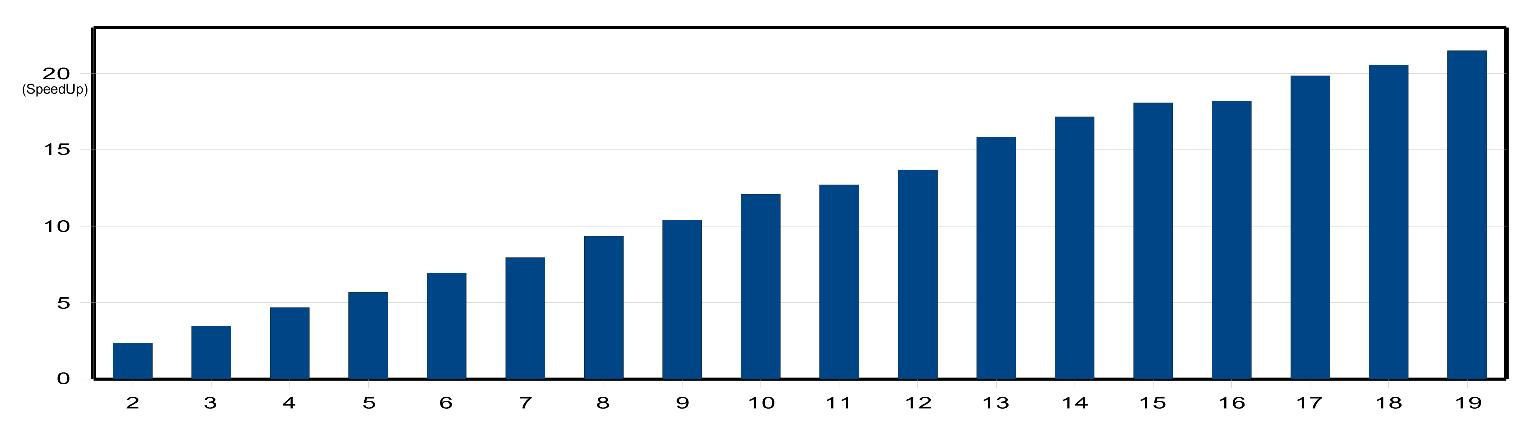
\includegraphics[width=12cm]{./../img/recogspeedup_300.eps}
\fi
\caption{Przykład przedstawia Lorem ipsum dolor sit amet (kolor niebieski)}
\label{class_selection}
\end{figure}

Przykładowe wartości statystyczne obliczone z histogramu dla wybranych obszarów: tło, brzeg komórki, wnętrze komórki przedstawione są w tabeli \ref{texture-feat-histogram}.
\begin{center}
\begin{table}[htb]	%[htb]
\label{texture-feat-histogram}
\caption{Przykładowe wartości statystyczne obliczone z histogramu dla wybranych obszarów.}
%\newcolumntype{S}{>{\centering\arraybackslash} m{.4\linewidth} }
\begin{tabular}{|c|c|c|c|c|}
\hline
\multicolumn{5}{c}{Wnętrze komórki} \\ \hline
Obraz obszaru & średnia & wariancja & skośność & kurtoza \\ \hline

\includegraphics[width=2cm]{./../img/texture-feats-examples/internal/lspot-0163-0202.eps}
	& 0.63137976 & 0.34081793 & 0.21212126 & -2.98348491 \\ \hline

\includegraphics[width=2cm]{./../img/texture-feats-examples/internal/lspot-0258-0153.eps}	
	& 0.60025141 & 0.32051886 & 0.19296321 & -2.98727716 \\ \hline
\multicolumn{5}{c}{Krawędź komórki} \\ \hline
Obraz obszaru & średnia & wariancja & skośność & kurtoza \\ \hline

\includegraphics[width=2cm]{./../img/texture-feats-examples/edge/lspot-0074-0134.eps}
	& 0.49186311 & 0.21801289 & 0.10819958 & -2.99728385 \\ \hline

\includegraphics[width=2cm]{./../img/texture-feats-examples/edge/lspot-0294-0093.eps}
	& 0.50519031 & 0.22901042 & 0.11651124 & -2.99668923 \\ \hline
\multicolumn{5}{c}{Tło} \\ \hline
Obraz obszaru & średnia & wariancja & skośność & kurtoza \\ \hline

\includegraphics[width=2cm]{./../img/texture-feats-examples/bkg/lspot-0420-0162.eps}
	& 0.49653979 & 0.21544670 & 0.10645873 & -2.99738607 \\ \hline

\includegraphics[width=2cm]{./../img/texture-feats-examples/bkg/lspot-0426-0189.eps}
	& 0.53896788 & 0.24888885 & 0.13234195 & -2.99531207 \\ \hline
\end{tabular}
\end{table}
\end{center}
%\clearpage

Proszę zwrócić uwagę na algorytm \ref{cooccurrence-algorithm}.

\begin{algorithm}
	\SetKwInOut{Input}{wejście}\SetKwInOut{Output}{wyjście}
	\Input{macierz $R$ o rozmiarze $rows\times columns$}
	\Output{macierze współwystępowania $C$}
	\BlankLine
	\For{$d\leftarrow 1$ \KwTo $distance$}
	{
		\ForEach{$\theta \in 0, \frac{2\pi}{dirs}, 2\pi$}
		{
%			\emph{zerowanie tablicy}\\
			\For{$i\leftarrow 0$ \KwTo $max~brightness$}
			{
				\For{$j\leftarrow 0$ \KwTo $max~brightness$}
				{
					$P_{d,\theta}(i, j) \leftarrow 0$\;
				}
			}
			\For{$t\leftarrow 0$ \KwTo $columns-1$}
			{
				\For{$k\leftarrow 0$ \KwTo $rows-1$}
				{
					$tc \leftarrow $floor$(t + d\cdot cos(\theta))$\;
					$kc \leftarrow $floor$(k + d\cdot sin(\theta))$\;
					\If{$(0 \leq yc)\cdot(yc < rows)\cdot(0 \leq xc)\cdot(xc < columns)$}
					{
						$C_{d,\theta}(R_{t,k},R_{tc,kc}) \leftarrow C_{d, \theta}(R_{t,k},R_{tc, kc}) + 1$\;
					}
				}
			}
		}
	}
\caption{Wyznaczanie macierzy współwystępowania}
\label{cooccurrence-algorithm}
\end{algorithm}

Po uzyskaniu macierzy współwystępowania generowane są następujące cechy:

\begin{equation}
\mu_{x} = \displaystyle\sum\limits_{m} m \displaystyle\sum\limits_{n} C_{d,\theta}(m,n)
\end{equation}

\begin{equation}
\mu_{y} = \displaystyle\sum\limits_{n} n \displaystyle\sum\limits_{m} C_{d,\theta}(m,n)
\end{equation}

\begin{equation}
\sigma_{x} = \displaystyle\sum\limits_{m}(m-\mu_x)^2 \displaystyle\sum\limits_{n} C_{d,\theta}(m,n)
\end{equation}

\begin{equation}
\sigma_{y} = \displaystyle\sum\limits_{n}(n-\mu_y)^2 \displaystyle\sum\limits_{m} C_{d,\theta}(m,n)
\end{equation}

\begin{equation}
Energy = \displaystyle\sum\limits_{m,n} C_{d,\theta}(m,n)^2
\end{equation}

\begin{equation}
Entropy = -\displaystyle\sum\limits_{m,n} C_{d,\theta}(m,n)\log(C_{d,\theta}(m,n))
\end{equation}

\begin{equation}
IDM = \displaystyle\sum\limits_{m,n}\frac{1}{1 + (m - n)^2} C_{d,\theta}(m,n)
\end{equation}

\begin{equation}
Shade = \displaystyle\sum\limits_{m,n}(m + n - \mu_x - \mu_y)^3 C_{d,\theta}(m,n)
\end{equation}

\begin{equation}
Inertia = \displaystyle\sum\limits_{m,n}(m-n)^2 C_{d,\theta}(m,n)
\end{equation}

\begin{equation}
Promenance = \displaystyle\sum\limits_{m,n}(m+n-\mu_x-\mu_y)^4 C_{d,\theta}(m,n)
\end{equation}

\begin{equation}
Correlation = -\displaystyle\sum\limits_{m,n}\frac{(m-\mu_x)(n-\mu_y)}{\sqrt{(\sigma_x \sigma_y)}} C_{d,\theta}(m,n)
\end{equation}

Do tej pory nie rozwiązywano w ten sposób problemu, zatem propozycja autora niniejszej rozprawy jest nowatorska \cite{SanFrancisco-poster}. 
